\begin{tikzpicture}[
    scale=1.1,
    every node/.style={font=\footnotesize},
    every path/.append style={line cap=round}
]

\begin{scope}[shift={(0.5,0.25)}]
\draw[myblue, thick, ->] (-4,0) -- (-3,0);
\draw[myblue] (-3.7,-0.4) -- (-3.7,0.4);
\draw[myblue] (-3.5,-0.4) -- (-3.5,0.4) node[above] {onde incidente};
\draw[myblue] (-3.3,-0.4) -- (-3.3,0.4);
\end{scope}

\node[anchor=south west, inner sep=0] (obs) at (0,0) {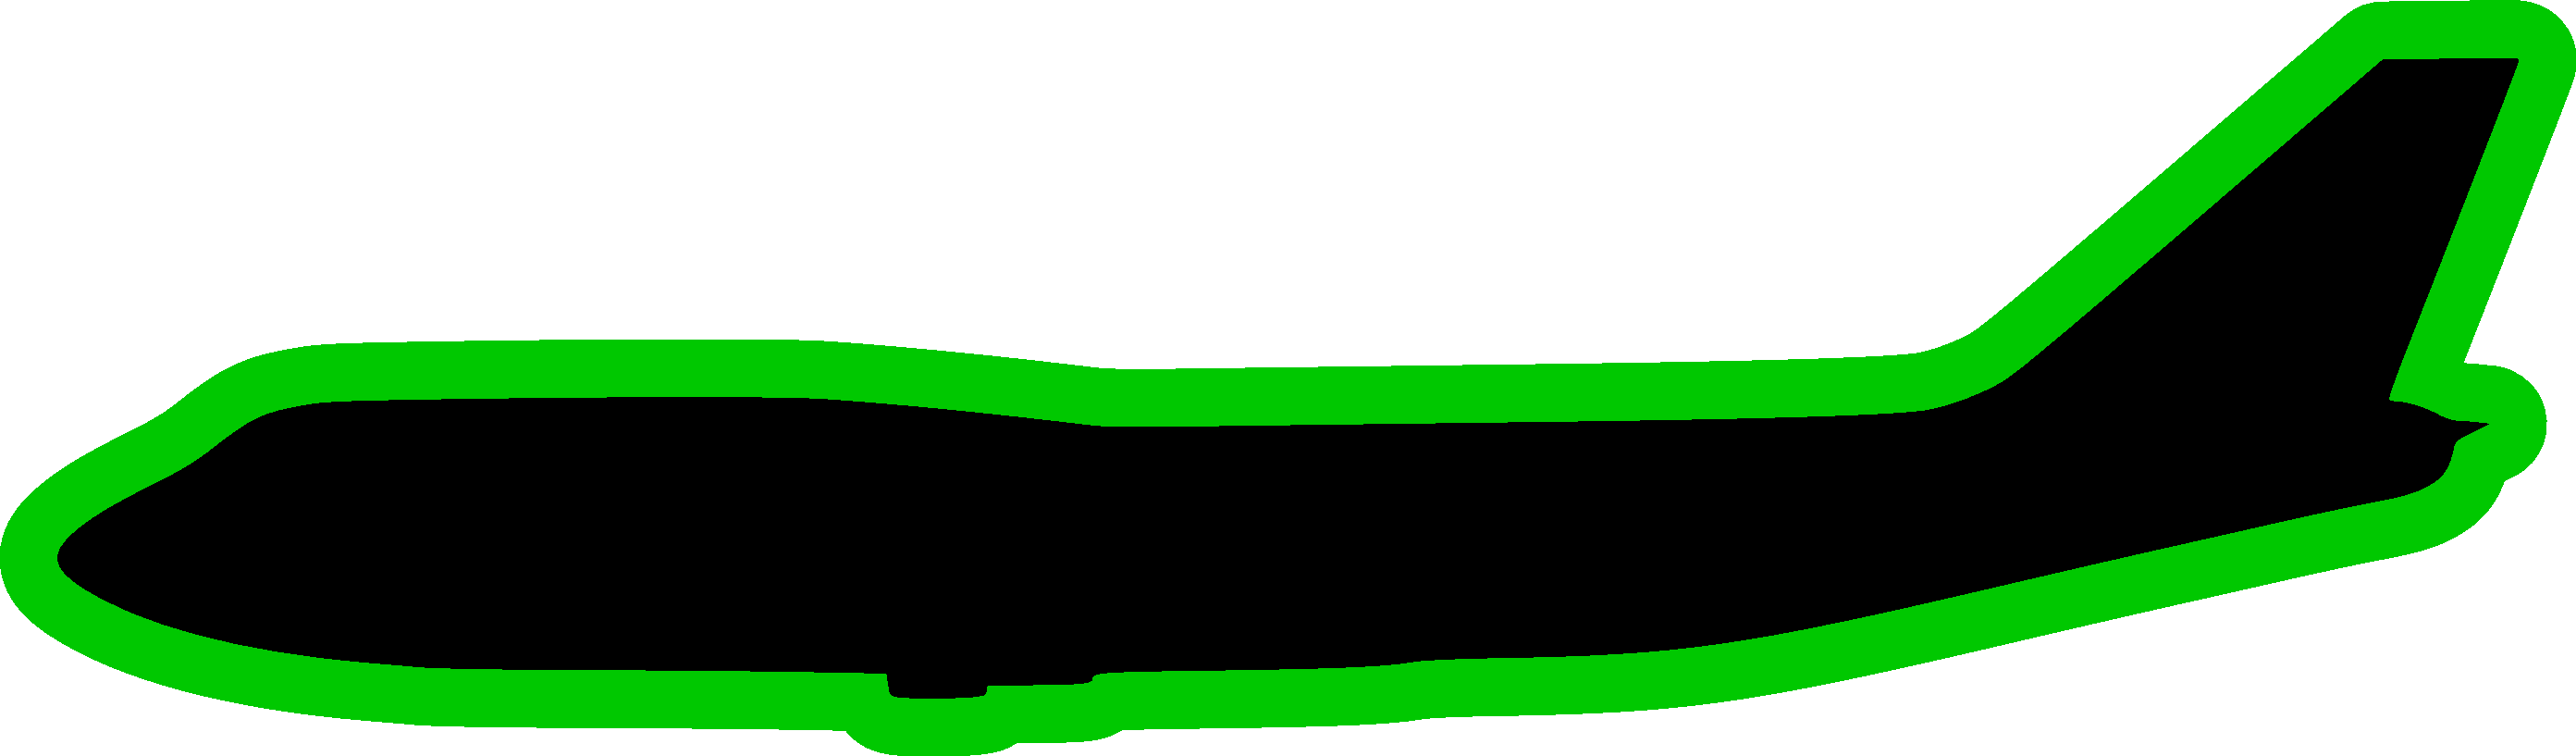
\includegraphics[width=2cm]{img/avion.pdf}};
\node[below=8pt] at (obs.center) {obstacle};
\node[mydarkgreen, right] at (obs.east) {$\Sigma$};

\begin{scope}[rotate=-45, shift={(0.03,0.25)}]
    \draw[decoration={expanding waves, segment length=3mm, angle=40}, decorate, myred] (0, 0) -- ++(-1.2,0) node[right=25pt] {onde diffractée};
    \draw[myred, thick, ->] (-0.2,0) -- (-1.3,0);
    \draw[myred, thick, ->, rotate around={-25:(0,0)}] (-0.2,0) -- (-1.3,0);
    \draw[myred, thick, ->, rotate around={25:(0,0)}] (-0.2,0) -- (-1.3,0);
\end{scope}

\end{tikzpicture}